\documentclass[a4paper,12pt]{article}
\usepackage{amsmath}
\usepackage{graphicx}
\usepackage{siunitx}
\usepackage{float}
\usepackage[hidelinks]{hyperref}

\title{Determination of the Molar Enthalpy of Neutralization}
\author{Group 304: Simone Keldenich (445904), Lukas Othman (446359), \\Kilian Mandon (445233)}
\date{18.09.2024}

\begin{document}

\maketitle
\newpage

\section{Introduction}
The enthalpy of neutralization (\(\Delta H_{\text{neutralization}}\)) is a fundamental thermodynamic quantity that measures the heat released when an acid and a base react to form water under standard conditions. For a strong acid-strong base reaction, this process can be represented as:
\begin{equation}
\text{H}^+ + \text{OH}^- \rightarrow \text{H}_2\text{O}
\end{equation}
In such reactions, both the acid and base dissociate completely in solution, resulting in the enthalpy change being a measure of the heat produced per mole of water formed. 

In this experiment, we aim to determine the molar reaction enthalpy of the neutralization of hydrochloric acid (HCl) with sodium hydroxide (NaOH) using a calorimetric approach. Additionally, we will evaluate the dilution heat effect to obtain the actual neutralization enthalpy by separating it from the heat absorbed due to the dilution of the acid.

The process is monitored using a calorimeter, which measures the temperature change associated with the reaction. By calibrating the calorimeter with electrical heating, we can accurately determine the heat capacity of the system, enabling us to calculate the enthalpy change based on temperature variations during the neutralization and dilution experiments. Error propagation analysis will be used to determine the uncertainties associated with the measurements.

\section{Methods}
\subsection{Preparation of Hydrochloric Acid Solution}
A hydrochloric acid solution of approximately 2.0 to 2.25 mol/L was prepared by diluting 17.5~mL concentrated HCl (37\% by mass, density = 1.19 kg/L) with deionized water to a final volume of 100 mL. The precise concentration of the resulting solution was determined using a titration method with a standardized 0.5 mol/L sodium hydroxide (NaOH) solution. 

Four titration measurements were performed, but only the last two were used for concentration determination due to observed inconsistencies with the first two values.

\subsection{Neutralization Experiment}
The calorimeter setup used for the neutralization experiment consisted of a Dewar flask to minimize heat exchange with the environment, a stirring mechanism to ensure uniform mixing, and a thermocouple connected to an ice-water reference point for accurate temperature measurements.

The experiment involved dissolving 1.866 g of NaOH pellets in 50 mL of deionized water directly inside the calorimeter. Additional deionized water was added to reach a specific marked volume. This process ensures that the heat produced during neutralization could be measured effectively.

To monitor the neutralization reaction, 20.00 mL of the prepared HCl solution was carefully transferred into a vessel, weighed, and its exact mass recorded. The HCl solution was then added to the NaOH solution within the calorimeter, and the temperature change was recorded for 5 minutes prior to the addition (pre-reaction period), during the reaction, and for an additional 5 minutes post-reaction.

\subsection{Calibration Experiment}
To accurately determine the heat capacity (\(C_W\)) of the calorimeter, a calibration experiment was conducted using electrical heating. A known voltage and current were applied to a heating element submerged in the calorimeter for 35 seconds. 

The electrical work supplied (\(W^*\)) was calculated using:
\begin{equation}
W^* = U \cdot I \cdot t,
\end{equation}
where \(U\) and \(I\) are the voltage and current values, and \(t = 35.0 \, s\) represents the heating duration. This allowed for the determination of the calorimeter's water value \(C_W\) through the relationship:
\begin{equation}
C_W = \frac{W^*}{\Delta T_{\text{calibration}}},
\end{equation}
where \(\Delta T_{\text{calibration}}\) is the measured temperature change during the calibration.

Since the thermoelectric potential change \(\Delta \Phi\) is directly proportional to the temperature change (\(\Delta T \sim \Delta \Phi\)), this calibration enables us to calculate the enthalpy changes for the neutralization and dilution experiments using their corresponding \(\Delta \Phi\) values.

\subsection{Dilution Experiment}
To account for the heat of dilution, the experiment was repeated using the same 20.00 mL of HCl solution, but without adding NaOH to the calorimeter beforehand. This allowed us to measure the heat associated solely with the dilution process, thereby enabling the separation of the dilution heat from the total measured heat in the primary neutralization experiment.

The thermoelectric potential change was recorded for 5 minutes pre-addition, during addition, and for an additional 5 minutes post-addition, similar to the neutralization experiment. This value was subtracted from the total heat measured during the neutralization to isolate the enthalpy of the neutralization reaction.

\subsection{Data Evaluation and Error Analysis}
The data collected during the experiments were analyzed to determine the molar reaction enthalpy (\(\Delta H_{\text{neutralization}}\)) and its associated error using Gaussian error propagation.

For the neutralization experiment, the change in temperature was determined graphically, with linear regressions fitted to different phases of the experiment (pre-reaction, post-reaction, and post-calibration periods). This method helped account for the fact that the calorimeter system is not perfectly isolated. By evaluating the difference between the linear equations at the chosen transition point, we obtained an approximation of the instantaneous temperature change that would have occurred in an ideally isolated system.

The molar enthalpy was calculated using:
\begin{equation}
\Delta H_{\text{molar}} = -\frac{W^* \cdot \Delta \Phi_{\text{neutralization}}}{\Delta \Phi_{\text{calibration}} \cdot n_{\text{acid}}},
\end{equation}
where \(\Delta \Phi_{\text{neutralization}}\) and \(\Delta \Phi_{\text{calibration}}\) are the potential differences observed during the neutralization and calibration experiments, respectively, and \(n_{\text{acid}}\) is the number of moles of HCl used.

Error propagation followed standard Gaussian methods, ensuring accurate reporting of uncertainties throughout the experiment.


\section{Results}
The results of this experiment include the determination of the concentration of the acid solution, the calibration of the calorimeter, and the calculation of the molar enthalpy of neutralization and dilution. 

\subsection{Titration Results}
The concentration of the hydrochloric acid solution was determined via titration. The titration volumes of the sodium hydroxide solution measured during the experiment were:
\begin{align*}
V_{\text{NaOH, 1}} &= 43.13 \, \text{mL}, \quad V_{\text{NaOH, 2}} = 40.59 \, \text{mL}, \\ \quad V_{\text{NaOH, 3}} &= 42.42 \, \text{mL}, \quad V_{\text{NaOH, 4}} = 42.11 \, \text{mL}
\end{align*}
As the first value was invalid, and the second appeared as an outlier, only the last two values were used for analysis.

The mean titration volume is calculated as:
\[
\bar{V}_{\text{NaOH}} = \frac{42.42 + 42.11}{2}\,\text{mL} = 42.265 \, \text{mL}
\]
The error in the mean titration volume was calculated by combining both statistical and systematic error components. The statistical error was estimated using the standard deviation of the measured values as an approximation, while a systematic error of \(0.05 \, \text{mL}\) was assumed based on the accuracy limitations of the semi-automatic burette used for the experiment.

The total error was then calculated using the formula:
\[
\sigma_{V_{\text{NaOH}}} = \sqrt{\frac{s_{\text{rand}}^2}{n} + s_{\text{sys}}^2}
\]
where \( s_{\text{rand}} \) represents the standard deviation of the measured volumes and \( s_{\text{sys}} = 0.05 \, \text{mL} \) accounts for the systematic error. For this experiment, with two valid measurements, \( n = 2 \), the calculation was performed as follows:

\[
s_{\text{rand}} = \sqrt{\frac{(42.42 - 42.265)^2 + (42.11 - 42.265)^2}{2-1}} \,\text{mL}= 0.219 \, \text{mL}
\]
Thus,
\[
\sigma_{V_{\text{NaOH}}} = \sqrt{\frac{0.219^2}{2} + 0.05^2} = 0.17 \, \text{mL}
\]
The total error in the mean titration volume was therefore determined to be \(0.17 \, \text{mL}\).
Thus, the mean volume and its error are:
\[
\bar{V}_{\text{NaOH}} = 42.27 \pm 0.17 \, \text{mL}
\]

The concentration of HCl, \( c_{\text{HCl}} \), is calculated from the known concentration of NaOH (\( c_{\text{NaOH}} = 0.5 \, \text{mol/L} \)):
\[
c_{\text{HCl}} = \frac{c_{\text{NaOH}} \cdot \bar{V}_{\text{NaOH}}}{V_{\text{HCl}}} = \frac{0.5 \cdot 42.27}{10.0} \,\si{\mol\per\litre}= 2.113 \, \si{\mol\per\litre}
\]
The propagated error for \( c_{\text{HCl}} \) is calculated as:
\[
\sigma_{c_{\text{HCl}}} = c_{\text{HCl}} \sqrt{\left(\frac{\sigma_{V_{\text{NaOH}}}}{\bar{V}_{\text{NaOH}}}\right)^2 + \left(\frac{\sigma_{V_{\text{HCl}}}}{V_{\text{HCl}}}\right)^2}
\]
Substituting \( \sigma_{V_{\text{HCl}}} = 0.05 \, \text{mL} \), the result is:
\[
\sigma_{c_{\text{HCl}}} = 0.014 \, \si{\mol\per\litre}
\]
Thus, the final concentration is:
\[
c_{\text{HCl}} = 2.113 \pm 0.014 \, \si{\mol\per\litre}
\]

\subsection{Calibration Experiment}
The calibration involved measuring the thermoelectric potential change during electrical heating, with voltage \( U \) ranging between 225 V and 230 V and current \( I \) ranging between 0.364 A and 0.375 A. The mean values were calculated as:
\[
U = \frac{225 + 230}{2} \,\text{V} = 227.5 \, \text{V}, \quad I = \frac{0.364 + 0.375}{2} \,\text{A}= 0.370 \, \text{A}
\]
The associated errors were:
\[
\sigma_U = \frac{230 - 225}{2} \,\si{\volt}= 2.5 \, \text{V}, \quad \sigma_I = \frac{0.375 - 0.364}{2} \,\si{\ampere}= 0.006 \, \text{A}
\]
The work \( W^* \) was calculated as:
\[
W^* = U \cdot I \cdot t = 227.5 \,\text{V}\cdot 0.370 \,\text{A}\cdot 35.0 \,\text{s}= 2942.14 \, \text{J}
\]
The propagated error for \( W^* \) is:
\[
\sigma_{W^*} = W^* \sqrt{\left(\frac{\sigma_U}{U}\right)^2 + \left(\frac{\sigma_I}{I}\right)^2 + \left(\frac{\sigma_t}{t}\right)^2}
\]
Substituting values, including an error of \( \sigma_t = 0.2 \, s \) as an estimate of the reaction time when operating the device:
\[
\sigma_{W^*} = 57 \, \text{J}
\]
Thus, the electrical work is:
\[
W^* = 2.94 \pm 0.06 \, \text{kJ}
\]

\subsection{Neutralization Experiment}
The mass of the HCl solution was determined from the weight difference before and after transfer:
\[
m_{\text{HCl}} = 86.295 \, \text{g} - 65.704 \, \text{g} = 20.591 \, \text{g}
\]

The error in the mass difference was calculated using an assumed weighing error of \(0.0005 \, \text{g}\) for each measurement. As the total mass difference involves two separate measurements, the error propagation formula yields:
\[
\sigma_{m_{\text{HCl}}} = \sqrt{2} \cdot 0.0005 \, \text{g} = 0.0007 \, \text{g}
\]

Given the density of the HCl solution, \( \rho_{\text{HCl}} = 1.03 \, \text{g/mL} \), the volume of HCl, \( V_{\text{HCl}} \), was calculated as:
\[
V_{\text{HCl}} = \frac{m_{\text{HCl}}}{\rho_{\text{HCl}}} = \frac{20.591 \,\si{\gram}}{1.03\,\si{\gram\per\milli\litre}} = 19.9913 \, \text{mL}
\]

The propagated error in \( V_{\text{HCl}} \), assuming no error on the density, was determined by dividing the mass error by the density:
\[
\sigma_{V_{\text{HCl}}} = \frac{\sigma_{m_{\text{HCl}}}}{\rho_{\text{HCl}}} = \frac{0.0007\,\si{\gram}}{1.03\,\si{\gram\per\milli\litre}} = 0.0007 \, \text{mL}
\]

Therefore, the volume of the HCl solution was determined to be:
\[
V_{\text{HCl}} = 19.9913 \pm 0.0007 \, \text{mL}
\]

The molar amount of HCl is:
\[
n_{\text{HCl}} = c_{\text{HCl}} \cdot V_{\text{HCl}} = 2.113 \,\si{\mol\per\litre}\cdot 19.991\,\si{\milli\litre} = 0.04225 \, \text{mol}
\]
The propagated error is:
\[
\sigma_{n_{\text{HCl}}} = n_{\text{HCl}} \sqrt{\left(\frac{\sigma_{c_{\text{HCl}}}}{c_{\text{HCl}}}\right)^2 + \left(\frac{\sigma_{V_{\text{HCl}}}}{V_{\text{HCl}}}\right)^2}
\]
Resulting in:
\[
\sigma_{n_{\text{HCl}}} = 0.00027 \, \text{mol}
\]
Thus,
\[
n_{\text{HCl}} = 0.04225 \pm 0.00027 \, \text{mol}
\]

\subsection{Graphical Evaluation of \(\Delta \Phi\) and Associated Errors}

The potential difference \(\Delta \Phi\) for both the neutralization and dilution experiments was determined using a graphical evaluation of the thermoelectric potential over time. This process involved fitting linear equations to different phases of the measured potential values to identify the transition points and calculate the \(\Delta \Phi\) values. The details for each experiment are outlined below.

\subsubsection{Neutralization Experiment}
The neutralization experiment was evaluated using the measured potential values recorded every minute. Three distinct phases were identified:
\begin{itemize}
    \item \textbf{Early phase:} [0, 5] minutes
    \item \textbf{Middle phase:} [6, 10] minutes
    \item \textbf{Late phase:} [18, 25] minutes
\end{itemize}

For each phase, a linear regression was fitted to the measured values. The transition point between the end of the first phase and the start of the second phase was determined by identifying the time at which the areas between the linear equation of the plateaus and the interpolated measured values on both the right-hand side (rhs) and left-hand side (lhs) of this point were equal. This was done using numerical integration, ensuring an accurate determination of the transition point.

The transition point was found to be at \(5.50 \, \text{min}\). The difference between the linear equations at this point provided the potential difference, \(\Delta \Phi_{\text{neutralization}}\), which was calculated as:
\[
\Delta \Phi_{\text{neutralization}} = 5.82 \cdot 10^{-5} \, \text{V}
\]

The error in \(\Delta \Phi_{\text{neutralization}}\) was determined from two components:
\begin{itemize}
    \item \textbf{Flat error:} This arises from error propagation through the difference of the linear equations. Given an error \(\phi_{\text{error}} = 1 \, \text{µV}\) on the function values, the flat error was calculated as:
    \[
    \sigma_{\text{flat}} = \sqrt{2} \cdot \phi_{\text{error}} = 1.41 \, \text{µV}
    \]
    \item \textbf{Positional error:} This was estimated by adjusting both linear equations up and down by \(\phi_{\text{error}}\) and checking the change in the transition point’s potential difference. The maximum absolute difference at these adjusted transition points was determined to be negligible in comparison to the flat error, at:
    \[
    \sigma_{\text{pos}} = 1.81 \cdot 10^{-8} \, \text{V}
    \]
\end{itemize}

Hence, the total error for \(\Delta \Phi_{\text{neutralization}}\) was:
\[
\sigma_{\Delta \Phi_{\text{neutralization}}} = 1.41 \, \text{µV}
\]

The final result for the neutralization potential difference is:
\[
\Delta \Phi_{\text{neutralization}} = 5.82 \cdot 10^{-5} \pm 0.15 \cdot 10^{-5} \, \text{V}
\]

The graphical evaluation for the neutralization and calibration experiments is shown in Figure \ref{fig:graphical_evaluation}.

\begin{figure}[H]
    \centering
    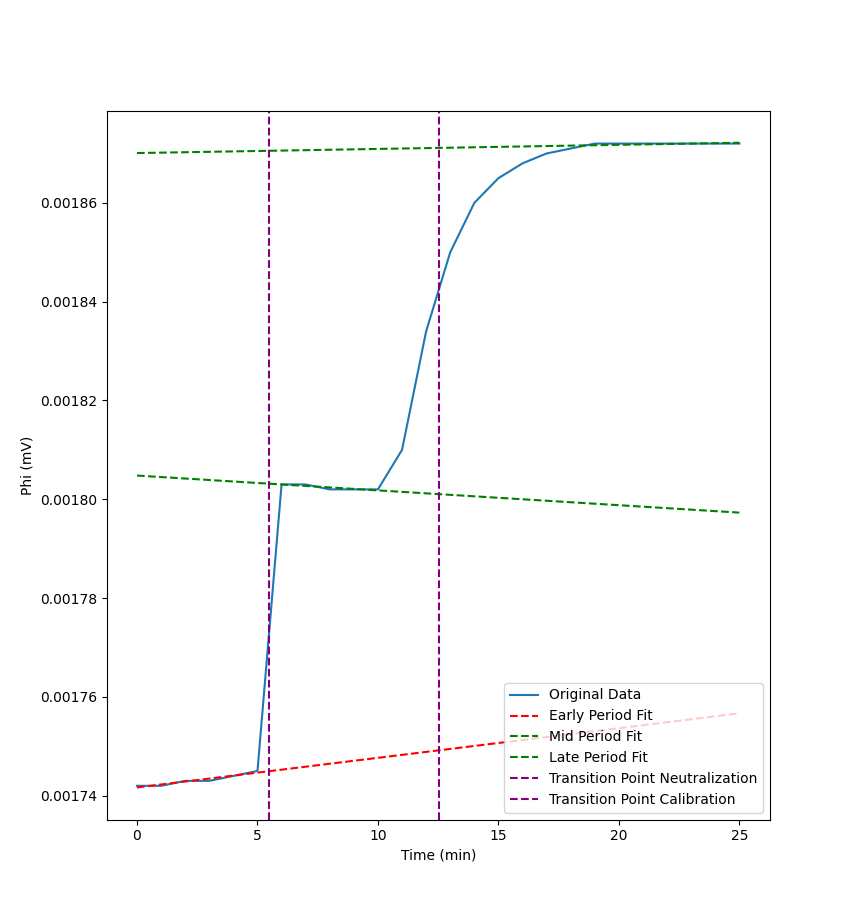
\includegraphics[width=\textwidth]{images/graphical_evaluation.png}
    \caption{Graphical evaluation of the thermoelectric potential change during the neutralization and calibration experiments. Linear fits for the early, middle, and late phases are displayed, along with the identified transition points.}
    \label{fig:graphical_evaluation}
\end{figure}

\subsubsection{Calibration Experiment}
A similar procedure was used to evaluate the calibration experiment. The transition point was determined at \(12.53 \, \text{min}\), resulting in a potential difference:
\[
\Delta \Phi_{\text{calibration}} = 7.01 \cdot 10^{-5} \, \text{V}
\]
The total error was calculated using the same method as in the neutralization experiment:
\[
\sigma_{\Delta \Phi_{\text{calibration}}} = 1.41 \, \text{µV}
\]
Thus, the final value for the calibration potential difference is:
\[
\Delta \Phi_{\text{calibration}} = 7.01 \cdot 10^{-5} \pm 0.15 \cdot 10^{-5} \, \text{V}
\]

\subsubsection{Dilution Experiment}
The graphical evaluation for the dilution experiment was carried out manually on paper. The potential difference was determined using the same technique of linear regression fitting and area equalization. The estimated transition point yielded a potential difference of:
\[
\Delta \Phi_{\text{dilution}} = 0.001685 - 0.0016822 V = 2.80 \cdot 10^{-6} \, \text{mV}
\]
The error in this value was assumed to be dominated by the flat error component:
\[
\sigma_{\Delta \Phi_{\text{dilution}}} = \sqrt{2} \cdot \phi_{\text{error}} = 1.41 \, \text{µV}
\]

Therefore, the potential difference for the dilution experiment was:
\[
\Delta \Phi_{\text{dilution}} = 2.8 \cdot 10^{-6} \pm 1.5 \cdot 10^{-6} \, \text{mV}
\]

The handwritten analysis for the dilution experiment is attached at the end of this document.

\subsection{Determination of Molar and Non-Molar Enthalpy}

The potential difference during the neutralization experiment was measured as:
\[
\Delta \Phi_{\text{neutralization}} = 5.82 \cdot 10^{-5} \pm 0.15 \cdot 10^{-5} \, \text{V}
\]

\subsubsection{Non-Molar Neutralization Enthalpy}
The total (non-molar) enthalpy change during neutralization was calculated using:
\[
\Delta H_{\text{neutralization}} = -\frac{W^* \cdot \Delta \Phi_{\text{neutralization}}}{\Delta \Phi_{\text{calibration}}} = -\frac{2942 \cdot 5.82 \cdot 10^{-5}}{7.01 \cdot 10^{-5}} \, \si{\joule}
\]
Substituting the values, we find:
\[
\Delta H_{\text{neutralization}} = -2442 \, \si{\joule}
\]
The error propagation for \(\Delta H_{\text{neutralization}}\) is given by:
\[
\sigma_{\Delta H_{\text{neutralization}}} = \Delta H_{\text{neutralization}} \cdot \sqrt{\left(\frac{\sigma_{W^*}}{W^*}\right)^2 + \left(\frac{\sigma_{\Delta \Phi_{\text{neutralization}}}}{\Delta \Phi_{\text{neutralization}}}\right)^2 + \left(\frac{\sigma_{\Delta \Phi_{\text{calibration}}}}{\Delta \Phi_{\text{calibration}}}\right)^2}
\]
Substituting the errors yields:
\[
\sigma_{\Delta H_{\text{neutralization}}} = 0.10 \, \si{\kilo\joule}
\]
Thus, the total non-molar enthalpy change is:
\[
\Delta H_{\text{neutralization}} = -2.44 \pm 0.10 \,\si{\kilo\joule}
\]

\subsubsection{Molar Neutralization Enthalpy}
The molar enthalpy change was calculated using:
\[
\Delta H_{m, \text{neutralization}} = \frac{\Delta H_{\text{neutralization}}}{n_{\text{HCl}}} = \frac{-2442\,\si{\joule}}{0.04225\,\si{\mol}} = -57816 \, \si{\joule\per\mol}
\]
The error propagation yields:
\[
\sigma_{\Delta H_{m, \text{neutralization}}} = \Delta H_{m, \text{neutralization}} \cdot \sqrt{\left(\frac{\sigma_{\Delta H_{\text{neutralization}}}}{\Delta H_{\text{neutralization}}}\right)^2 + \left(\frac{\sigma_{n_{\text{HCl}}}}{n_{\text{HCl}}}\right)^2}
\]
Resulting in:
\[
\sigma_{\Delta H_{m, \text{neutralization}}} = 2170 \, \si{\joule\per\mol} = 2.17 \, \si{\kilo\joule\per\mol}
\]
Therefore, the molar neutralization enthalpy is:
\[
\Delta H_{m, \text{neutralization}} = -57.8 \pm 2.2 \, \si{\kilo\joule\per\mol}
\]

\subsubsection{Non-Molar and Molar Dilution Enthalpy}
The potential difference during the dilution experiment was determined as:
\[
\Delta \Phi_{\text{dilution}} = 2.80 \cdot 10^{-6} \pm 1.41 \cdot 10^{-6} \, \text{V}
\]
The non-molar enthalpy change for dilution is calculated using:
\[
\Delta H_{\text{dilution}} = -\frac{W^* \cdot \Delta \Phi_{\text{dilution}}}{\Delta \Phi_{\text{calibration}}} = -\frac{2942 \cdot 2.80 \cdot 10^{-6}}{7.01 \cdot 10^{-5}} \, \si{\joule}
\]
Substituting the values, we get:
\[
\Delta H_{\text{dilution}} = -118 \, \si{\joule}
\]
The error propagation yields:
\[
\sigma_{\Delta H_{\text{dilution}}} = \Delta H_{\text{dilution}} \cdot \sqrt{\left(\frac{\sigma_{W^*}}{W^*}\right)^2 + \left(\frac{\sigma_{\Delta \Phi_{\text{dilution}}}}{\Delta \Phi_{\text{dilution}}}\right)^2 + \left(\frac{\sigma_{\Delta \Phi_{\text{calibration}}}}{\Delta \Phi_{\text{calibration}}}\right)^2}
\]
Resulting in:
\[
\sigma_{\Delta H_{\text{dilution}}} = 0.06 \, \si{\kilo\joule}
\]
Thus, the total non-molar dilution enthalpy is:
\[
\Delta H_{\text{dilution}} = -0.12 \pm 0.06 \, \si{\kilo\joule}
\]

The molar dilution enthalpy is then:
\[
\Delta H_{m, \text{dilution}} = \frac{\Delta H_{\text{dilution}}}{n_{\text{HCl}}} = \frac{-118\,\si{\joule}}{0.04225\,\si{\mol}} = -2782 \, \si{\joule\per\mol}
\]
The propagated error is:
\[
\sigma_{\Delta H_{m, \text{dilution}}} = \Delta H_{m, \text{dilution}} \cdot \sqrt{\left(\frac{\sigma_{\Delta H_{\text{dilution}}}}{\Delta H_{\text{dilution}}}\right)^2 + \left(\frac{\sigma_{n_{\text{HCl}}}}{n_{\text{HCl}}}\right)^2}
\]
Resulting in:
\[
\sigma_{\Delta H_{m, \text{dilution}}} = 1.41 \, \si{\kilo\joule\per\mol}
\]
Thus,
\[
\Delta H_{m, \text{dilution}} = -2.8 \pm 1.5 \, \si{\kilo\joule\per\mol}
\]

\subsubsection{Molar Difference Between Neutralization and Dilution Enthalpies}
The difference between the molar enthalpy changes is calculated as:
\begin{align*}
\Delta H_{m, \text{neutralization-dilution}} &= \Delta H_{m, \text{neutralization}} - \Delta H_{m, \text{dilution}} = -57.8 - (-2.78) \\ &= -55.0 \, \si{\kilo\joule\per\mol}
\end{align*}
The error propagation for this difference is:
\[
\sigma_{\Delta H_{m, \text{neutralization-dilution}}} = \sqrt{\sigma_{\Delta H_{m, \text{neutralization}}}^2 + \sigma_{\Delta H_{m, \text{dilution}}}^2}
\]
Substituting the values:
\[
\sigma_{\Delta H_{m, \text{neutralization-dilution}}} = \sqrt{(2.17)^2 + (1.41)^2} \,\si{\kilo\joule\per\mol}= 2.6 \, \si{\kilo\joule\per\mol}
\]
Therefore, the final result for the molar difference is:
\[
\Delta H_{m, \text{neutralization-dilution}} = -55.0 \pm 2.6 \, \si{\kilo\joule\per\mol}
\]


\section{Discussion}
The primary objective of this experiment was to determine the molar enthalpy of neutralization for the reaction between hydrochloric acid (HCl) and sodium hydroxide (NaOH) and to compare it with theoretical and literature values. 

\subsection{Comparison with Reference Values}
The experimentally determined molar enthalpy of neutralization was found to be:
\[
\Delta H_{m, \text{neutralization}} = -57.8 \pm 2.2 \, \si{\kilo\joule\per\mol}
\]
This result aligns closely with the value provided by the lab tutorial instructor of \(-57.5 \, \si{\kilo\joule\per\mol}\). Given the overlap in uncertainties, this suggests that the experimental procedure was largely accurate in capturing the heat released during the neutralization of a strong acid and base.

Additionally, when compared to the theoretical formation enthalpy of liquid water from aqueous \(\text{H}^+\) and \(\text{OH}^-\), calculated using standard formation enthalpies from Atkins\footnote{Atkins, P. (2018). \textit{Physical Chemistry} (11th ed.). Oxford University Press.}, which is \(-55.84 \, \si{\kilo\joule\per\mol}\), the experimental value shows a slight deviation. The difference between our experimental value and the theoretical enthalpy can be partially attributed to the fact that our experiment also includes the heat of dilution, which can be significant.

By subtracting the measured dilution enthalpy \(\Delta H_{m, \text{dilution}} = -2.8 \pm 1.5 \, \si{\kilo\joule\per\mol}\) from the total neutralization enthalpy, we obtain a corrected value:
\[
\Delta H_{m, \text{neutralization-dilution}} = -55.0 \pm 2.6 \, \si{\kilo\joule\per\mol}
\]
This corrected value is very close to the theoretical enthalpy of formation of water \((-55.84 \, \si{\kilo\joule\per\mol})\). However, it should be noted that the relatively large error range, especially in the dilution measurement, limits the certainty of this agreement. Given this uncertainty, the precise contribution of the dilution effect to the overall neutralization enthalpy could not be definitively determined. Thus, while the corrected result appears to align well with the theoretical value, caution must be exercised in drawing firm conclusions.

\subsection{Error Analysis and Experimental Assumptions}
The accuracy of the experiment was influenced by several potential sources of error and assumptions made during the procedure:

\begin{itemize}
    \item \textbf{Assumption of a closed system:} One key assumption was that the calorimeter functioned as a perfectly closed system, preventing any heat exchange with the surroundings. In reality, heat loss to the environment is unavoidable, even with the use of a Dewar flask to minimize this effect. This potential heat loss could lead to a slight underestimation of the heat released during the reaction, introducing a source of error in the enthalpy measurements.

    \item \textbf{Non-constant heat capacity of the calorimeter:} Although we calibrated the calorimeter ourselves, the heat capacity (\(C_W\)) may not remain entirely constant throughout the experiment, especially if the temperature changes significantly. Variations in \(C_W\) would directly impact the calculated enthalpies, leading to inaccuracies. While our calibration ensured a baseline measurement, fluctuations in heat capacity during different phases of the experiment could still be a source of error.

    \item \textbf{Dominance of the error on \(\Delta \Phi\):} The graphical evaluation of \(\Delta \Phi\) involved fitting linear equations through different phases of the reaction. Although the exact positioning of the transition point had relatively little influence on the final result, the primary contributor to the overall error was the measurement uncertainty in \(\Delta \Phi\). Therefore, improving the precision of these voltage measurements would likely have the most significant impact on reducing the total error in the enthalpy determination.
\end{itemize}

In summary, the experiment yielded a molar enthalpy of neutralization that closely matched the expected value from the lab instructor and the theoretical value when corrected for dilution effects. However, given the inherent experimental uncertainties and assumptions, particularly regarding the calorimeter's heat loss and measurement precision, the influence of dilution could not be definitively separated from the neutralization process.

\subsection{Conclusion}
The experiment successfully determined the molar enthalpy of neutralization for a strong acid-base reaction, aligning with both experimental and theoretical expectations. Despite potential sources of error, the results demonstrate the reliability of calorimetric techniques in quantifying thermodynamic properties, albeit with the need for careful consideration of systematic and random errors.

\section{Acknowledgements and Disclosure}
This protocol was prepared with the assistance of ChatGPT, an AI language model developed by OpenAI. All content generated by ChatGPT, including text, equations, and calculations, was thoroughly reviewed and corrected by the authors where necessary to ensure accuracy.

All materials used in the creation of this protocol, including the Python evaluation scripts, LaTeX source code, and ChatGPT conversations, can be found on GitHub\footnote{\url{https://github.com/kilianmandon/pc_praktikum/tree/main/neutralization_enthalpy}}. These resources will be available for up to four weeks after the conclusion of the lab tutorial.

\newpage
\appendix
\section*{Appendix}

\subsection*{Calculation of the Necessary Volume of 37\% HCl}
To prepare a hydrochloric acid solution with a concentration between 2.0 and 2.25 mol/L, we start with concentrated HCl (37\% by mass, density = 1.19 g/mL). First, we calculate the mass of HCl in 1 liter of this concentrated solution:
\[
m_{\text{HCl}} = 0.37 \cdot 1.19\,\si{\gram\per\milli\litre} \cdot 1000 \, \text{mL} = 440.3 \, \text{g}
\]
The molar mass of HCl is approximately 36.46 g/mol, so the molarity \( c \) of the concentrated solution is:
\[
c = \frac{440.3}{36.46} \,\si{\mol\per\litre}\approx 12.08 \, \text{mol/L}
\]
To dilute this to a concentration of 2.0 to 2.25 mol/L, we calculate the required volume \( V_{\text{concentrated}} \) using the dilution formula \( c_1 V_1 = c_2 V_2 \):
\[
V_{\text{concentrated}} = \frac{c_2 \cdot V_2}{c_1} = \frac{2.0 \cdot 100}{12.08} \,\si{\milli\litre}\approx 16.6 \, \text{mL}
\]
Thus, to achieve the desired concentration range, between 16.6 mL and 18.6~mL of concentrated HCl should be diluted to a final volume of 100~mL with deionized water.

\subsection*{Calculation of NaOH Mass for Neutralization}
To neutralize the HCl solution in the calorimeter, we first determine the number of moles of HCl:
\[
n_{\text{HCl}} = c_{\text{HCl}} \cdot V_{\text{HCl}} = 2.113 \, \text{mol/L} \cdot 0.020 \, \text{L} = 0.0423 \, \text{mol}
\]
The molar mass of NaOH is approximately 40.00 g/mol, so the mass of NaOH needed for complete neutralization is:
\[
m_{\text{NaOH}} = n_{\text{HCl}} \cdot M_{\text{NaOH}} = 0.0423 \cdot 40.00 \,\si{\gram}= 1.69 \, \text{g}
\]
Including a 10\% excess, the total mass required is:
\[
m_{\text{NaOH, total}} = 1.69\,\si{\gram} \cdot 1.1 \approx 1.86 \, \text{g}
\]

\subsection*{Note on Experimental Data and Graphical Evaluation}
The following pages contain scanned copies of the experimental data recorded during the lab session, as well as the handwritten graphical evaluation performed for the dilution experiment.


\end{document}